\documentclass[aps,prl,reprint,groupedaddress]{revtex4-1}
\usepackage{graphicx}

\begin{document}

%Title of paper
\title{Simulation of a fluid in a pipe using a Lattice Boltzmann model}

\author{Fernando Agust\'in I\~niguez R\'abago}
\author{Eduardo Pavinato Olimpio}
\email[]{All files on https://github.com/epolimpio/lattice\_boltzmann}

\affiliation{ICCP - Delft University of Technology}

\date{\today}

\begin{abstract}
% insert abstract here
In this report we present the results of simulations of a fluid flowing in a pipe using a Lattice-Boltzmann Bhatnagar-Gross-Krook (BGK) model in a square (d2q9) lattice. The results obtained using a Poiseuille flow are successfully compared to the theory. Furthermore, we added an obstacle to the flow showing the potential of the model to simulate the flow across more complicated boundaries. 
\end{abstract}

\maketitle

% References should be done using the \cite, \ref, and \label commands 

\section{Lattice Boltzmann model}

The Lattice Boltzmann model uses a ``toy model'' for the liquid with discretization in time and space (the lattice). In each node of the lattice, instead of having particles as in the Lattice Gas Automata models, it uses densities to avoid fluctuations. The densities at each site have a particular velocity that allows it to move to another site every time step. We use the so called d2q9 square lattice for a two dimensional fluid, as indicated in figure \ref{lattice}.

\begin{figure}[hb]
	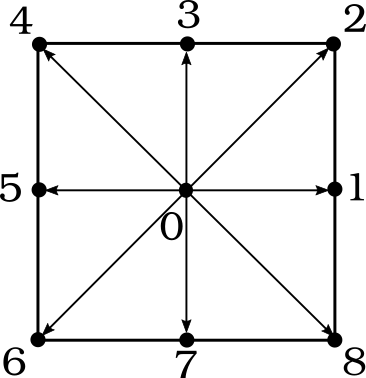
\includegraphics[scale=0.3]{array.png}
	\caption{Square lattice used in the Lattice Boltzmann model. At each node we have nine densities, each corresponding to one of the indicated velocity vectors (0 to 8). After relaxation, we move the corresponding density to its neighbour using this velocity. \label{lattice}}
\end{figure} 

The evolution is given by the Boltzmann equation, using Bhatnagar-Gross-Krook (BGK) approximation with a relaxation time $\tau$:

\begin{equation} \label{relax}
n_{i}(\mathbf{r}+c\Delta t\mathbf{e}_{i},t+\Delta t) = n_{i}(\mathbf{r},t)-\frac{1}{\tau}\left [n_{i}(\mathbf{r},t)-n_{i}^{eq}(\mathbf{r},t)  \right ]
\end{equation}
where we take $c$ and $\Delta t$, velocity and time step, respectively, as 1 for simplicity. The label $i$ denotes the 9 possible directions $\mathbf{e}_{i}$ on each site.  The equilibrium density is given by:

\begin{equation} \label{equil}
n_i^{eq} = w_i\frac{\rho}{m}\left(1+\frac{3}{c^2}e_{i\alpha}u_\alpha + \frac{9}{2c^4}e_{i\alpha}e_{i\beta}u_\alpha u_\beta - \frac{3}{2}\frac{u_\alpha u_\beta}{c^2}\right)
\end{equation}
where the labels $\alpha$ and $\beta$ are the Cartesian coordinates $x$ and $y$, the $w_i$ is a weight due to the grid ($4/9$ for $i=0$, $1/9$ for $i=1,3,5,7$, $1/36$ for $i=2,4,6,8$), $\rho = \sum_i n_i$ is the density at each site and $u_{\alpha} = c \sum_i n_i e_{i\alpha}$ is the average velocity on each site.

It can be shown \cite{ICCPBook} that under appropriate approximations (incompressible fluid, ideal gas relation and small Mach number), this system is equivalent to the Navier-Stokes equation for fluid dynamics, with viscosity $\nu = \frac{(2\tau + 1) \Delta x^2}{6 \Delta t}$. Using $c$ and $\Delta t$ equal to one, the velocities obtained are given in units of the sound velocity.

\section{Implementation}

The implementation of the Lattice Boltzmann model is done through the following algorithm:

\begin{enumerate}
\item Move the densities to the appropriate neighbor
\item Calculate velocities at each point
\item Apply the boundary conditions
\item Add a small velocity in the flow direction
\item Calculate the equilibrium densities
\item Relax the densities inside the system
\end{enumerate}

In the walls, we used the ``modified bounce back'' condition, where the zero slip boundary is between two node points. Although there is a small residual slip in the wall due to this implementation and better implementations could be performed \cite{He1997a}, we use this conditions by its simplicity and efficiency. This condition is implemented by inverting the velocity ($\vec{v} \to -\vec{v}$) of the densities that move into the wall nodes. In the inlet/outlet of the pipe we use periodic coundary conditions.

After calculating the average velocities on each site we add a small amount in the flowing direction. This is to impose a flow due to a constant pressure gradient. With this we calculate the equilibrium densities following the equation \ref{equil} to later relax the system according to equation \ref{relax}.

We run the algorithm until the system reaches equilibrium, what was checked by monitoring the average velocity in the center of the tube. We successfully used a grid of size $N_x$ between 50 and 500 and $N_y$ between 20 and 200, $\tau$ between $0.75$ and $20$ and the velocity added at each step between $10^{-2}$ and $10^{-7}$. The number of steps to reach equilibrium changes depending on the parameters and it tipically ranges between 1000 and 10000. Therefore we used 10000 timesteps for the simulations discussed in the next section. 

\begin{figure}[ht]
	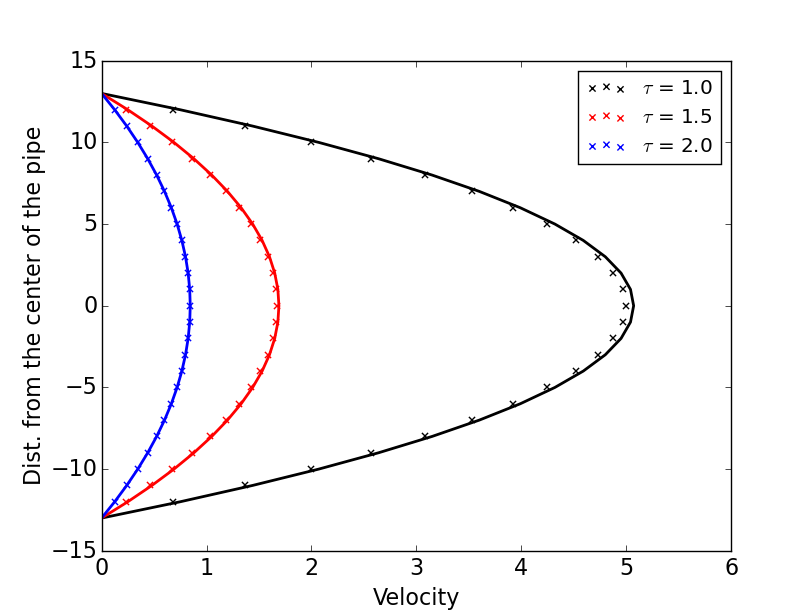
\includegraphics[scale=0.4]{poiseuille.png}
	\caption{Velocity profile of a Poiseuille flow simulated with the Lattice Boltzmann implementation (X markers) compared to the exact solution (lines) for fluids of different viscosities ($\nu = \frac{2\tau + 1}{6}$). The grid size for the simulation is $N_x \times N_y = 51 \times 27$ and the added velocity is $10^{-2}$. \label{poiseuille}}
\end{figure}

\section{Results}

First, we present the results of our simulation for the Poiseuille flow. In figure \ref{poiseuille} is shown the velocity profile on an axis perpendicular to the flow for fluids of different viscosities (represented by the relaxation time $\tau$). This is compared with the exact parabolic profile solution (Poiseuille flow), showing the agreement of the simulations with the theory. Although not presented here, we checked that the small differences seen between the exact and the simulated profiles are due to a bias in the boundary, as indicated by \cite{He1997a}.

Further, we added a triangular ladder obstruction in the pipe and let the system reach equilibrium. We used $N_x=101$ and $N_y=21$ to make the visualization of the results easier. We can see in figure \ref{arrows} that, according to the conservation laws the velocity increases as the diameter is constrained, reaching a maximum on the top of the ladder.

\begin{figure}[ht]
	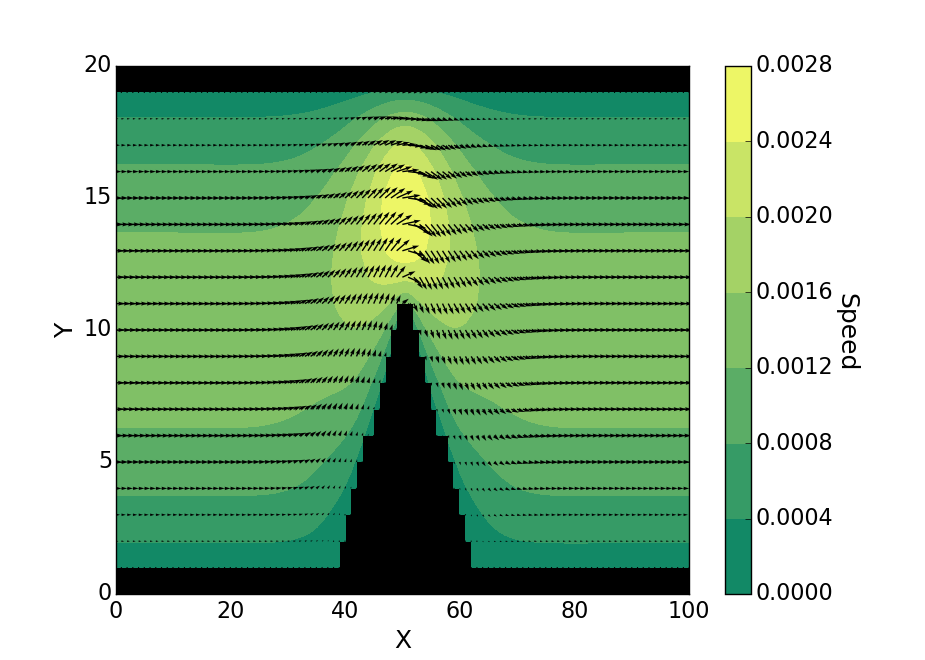
\includegraphics[scale=0.4]{arrows.png}
	\caption{Velocity map of a fluid through a pipe with a triangular ladder obstacle. The arrows indicate the velocity vectors. The grid size for the simulation is $N_x \times N_y = 101 \times 21$, the relaxation time is $\tau=1.0$ and the added velocity is $10^{-5}$. \label{arrows}}
\end{figure}

We also tested other obstacles, including blocks and circular objects. It is important to notice that the introduction of the obstacle increase the velocity in some regions and, therefore, the range of combinations of $\tau$ and pressure gradients for which the approximations are valid change. Because of that, we used a lower added velocity or higher viscosities ($\tau$) in this case.

\section{Conclusion \label{conclusion}}

In this report we show the implementation of a d2q9 Lattice-Boltzmann model and the results obtained for a flow in a pipe. The results indicate that the implementation can be further used in more complex boundaries. Further work will include the implementation of moving boundaries, using the idea presented in \cite{Kang2008}, and the extension of the model to three dimensions.
% Create the reference section using BibTeX:
\bibliography{Sciences}

\end{document}
